% IEEEAerospace2012.cls requires the following packages: times, rawfonts, oldfont, geometry
\documentclass[twocolumn,letterpaper]{IEEEAerospaceCLS}  % only supports two-column, letterpaper format

% The next line gives some packages you may find useful for your paper--these are not required though.
%\usepackage[]{graphicx,float,latexsym,amssymb,amsfonts,amsmath,amstext,times,psfig}
% NOTE: The .cls file is now compatible with amsmath!!!

\usepackage[]{graphicx}    % We use this package in this document
\usepackage{amsmath}
\usepackage{hyperref}
\hypersetup{
    colorlinks=true,
    linkcolor=black,
    filecolor=black,      
    urlcolor=black,
    citecolor=black,
    % draft,
}
\newcommand{\ignore}[1]{}  % {} empty inside = %% comment
\newcommand\todo[1]{\textbf{\textcolor{red}{#1}}}
\graphicspath{{imgs/}}

\begin{document}
\title{An ontology for UAV based  Semantic Navigation}

\author{%
    Nicolas Mandel\\
    Queensland University of Technology\\
    Australian Centre for Robotic Vision\\
    QUT Centre for Robotics\\
    nicolasjohann.mandel@hdr.qut.edu.au
    \and
    Michael Milford\\
    Queenslad University of Technology\\
    Nowhere, ZS 99999\\
    jane.smith@nowhere.edu
    \and
    Felipe Gonzalez\\
    Queenslad University of Technology\\
    Nowhere, ZS 99999\\
    jane.smith@nowhere.edu
    %%%% IMPORTANT: Use the correct copyright information--IEEE, Crown, or U.S. government. %%%%%
    \thanks{\footnotesize 978-1-7281-7436-5/21/$\$31.00$ \copyright2021 IEEE}              % This creates the copyright info that is the correct 2021 data.
    %\thanks{{U.S. Government work not protected by U.S. copyright}}         % Use this copyright notice only if you are employed by the U.S. Government.
    %\thanks{{978-1-7281-7436-5/21/$\$31.00$ \copyright2021 Crown}}          % Use this copyright notice only if you are employed by a crown government (e.g., Canada, UK, Australia).
    %\thanks{{978-1-7281-7436-5/21/$\$31.00$ \copyright2021 European Union}}    % Use this copyright notice is you are employed by the European Union.
}



\maketitle

\thispagestyle{plain}
\pagestyle{plain}



\maketitle

\thispagestyle{plain}
\pagestyle{plain}

\begin{abstract}
    Limitations in power, size and weight in UAVs have resulted in researchers exploring alternative navigation approaches to reduce the computational load onboard UAVs. In this work we present an ontology for semantic based navigation for UAVs. Contextual information is commonly used for navigation, with semantics at the frontier of contemporary robotic-based navigation research showing promising results. However, the connection between spatial and semantic information is not yet clear and formal definitions are limited in the literature. This paper aims to provide an ontology to link spatial and semantic relations through Ologs, an application of the mathematical field of category theory. Contemporary semantic concepts from natural language are fused with a spatial-semantic hierarchy in a mathematical framework. The framework is tested in simulations and its applicability verified with different scenarios. Results indicate that the defined spatial structure allows for improved UAV navigational capabilities. The presented ontology is mathematically sound and can be adapted to a number of semantic navigation use-cases in agriculture, search and rescue or industrial inspections.
\end{abstract}


\tableofcontents

%%%%%%%%%%%%%%%%%%%%%%%%%%%%%%%%%%%%%%
\section{Introduction} \label{sec:Intro}
%%%%%%%%%%%%%%%%%%%%%%%%%%%%%%%%%%%%%%

\subsection{Problem Introduction}

\subsection{Why is this problem important}
Contemporary robotics places great emphasis on including semantic signals into the perception-understanding-control-pipeline. Semantic information has been included into the passive part of SLAM~\cite{cadena_past_2016,zhang_hierarchical_2019}, as well as into the active decision~\cite{koch_automatic_2019,alirezaie_exploiting_2017}. Kostavelis and Gasteratos define semantics as " [...] related to the study between signs and the things to which they refer, that is their meaning."~\cite{kostavelis_semantic_2015}. However, in terms of spatial occurrence, multiple levels of signals are possible, such as individual objects, regions or areas~\cite{kostavelis_semantic_2015}. These s cause novel problems for definining successful navigation, as highlighted by Anderson et al.~\cite{anderson_evaluation_2018}. Furthermore, recent advances in Computer Vision have produced a wide range of different sensors signals to be annotated with semantic information, such as pixel-level segmentation, object detection or scene classification~\cite{alom_history_2018}, which operate on different spatial levels.\\
The influence of these novel signals on the level of names on conventional robotics algorithms, such as filters and path planners, is an active field of research. Furthermore, UAVs represent a special case of robotics, which are impacted by unique viewing angles, as well as risk-averse requirements.
\subsection{What do we propose for solving it}
In this paper we provide an overview of a selected subset of the literature on combining semantic signals with spatial information in robotics to illustrate the evolution of the field with novel algorithms information, specifically in the context of UAVs. First, we provide a brief overview of early approaches from the turn of the century. Second, we display a select subset of contemporary approaches, which include semantic information into novel algorithms. Third, we highlight approaches that incorporate semantic information into UAV pipelines.\\
In the second section we conduct numerical experiments on the well-defined problem of semantic mapping of a two-dimensional occupancy grid~\cite{gonzalez_unmanned_2016} and show how conventional parameters surrounding the quality of observations, overlap and field of view influence a naive bayesian filter. We supplement the filter through an informed prior and demonstrate the effectiveness and shortcomings of the approach. This research is directed towards enhancing the performance of a module which is tasked with understanding and evaluating the semantic information of a UAV as demonstrated by Mandel et al.~\cite{mandel_towards_2020}\\
As a future prospect, we briefly point to approaches from related semantic fields, such as speech recognition and language processing, which hold the potential to enhance the inclusion of semantic information.\todo{cite lienou - semantic annotation of satellite images using LDA}.

\section{Methodology} \label{sec:Met}
\subsection{Literature Review} \label{ssec:MetLit}
In this research a literature review of $22$ selected works has been conducted. These $22$ works, have been sorted according to the following dimensions:
\begin{enumerate}
    \item Robot Type
    \item Spatial Map Type
    \item Semantic Information
\end{enumerate}
The results of the literature overview are summarised in section~\ref{ssec:ResLit} and presented in a table in Appendix~\todo{Appendix naming}. The insights collected from the literature review are used to propose an adaption to generic semantic mapping algorithms to enhance the performance~\cite{kostavelis_semantic_2015}. Following the development pipeline as shown in figure~\ref{fig:DevProcess}, after the proposal of an algorithm, numerical simulations are conducted to highlight the improved performance. The results from the numerical simulation are presented in section~\ref{ssec:ResSim} and conclusions for future developments and potential integration into higher level architectures are drawn.
\subsection{Simulations} \label{ssec:MetSim}
\begin{figure}
    \centering
    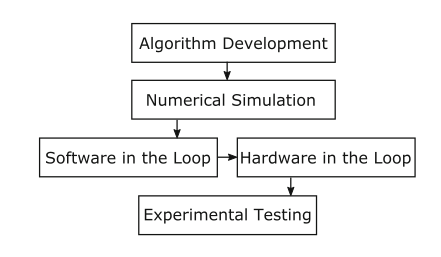
\includegraphics[width=3.25in]{2-3DevelopmentCycle}\\
    \caption{\bf{A generic autonomy development cycle as described by Ladosz et al.~\protect\cite{ladosz_generic_2019}}}
    \label{fig:DevProcess}
\end{figure}
Numerical simulations are conducted to uncover influences of parameters of the mapping pipeline and differences between algorithms. The task is concerned with recreating a map from noisy semantic observations. The map is an evenly spaced 2D grid $M \times M$ defined by a one-hot vector of the true identity, $x_{i,j} = \{0,..., 1, ..., 0\}_K$, with $K$ indicating the number of classes. The probability of making an observation $z$ is given by $p(z\mid x)$. The pose is assumed to be known for the entire trajectory. At each time increment $t$ the UAV observes cells within its field of view $f$, receives a one-hot observation proportional to $p(z\mid x)$ and updates the posterior of each map cell given by Bayes' rule as:
\begin{equation} \label{eq:Bayes}
    p(x\mid z) = \frac{p(z\mid x) p(x)}{p(z)}
\end{equation}
which is equivalent to the performance of any given detector~\cite{alom_history_2018}.
The UAV is following a conventional lawnmower pattern, where the stride in both dimensions is defined through a desired overlap $o$ and field of view $f$~\cite{shetty_implementation_2020}. Figure~\ref{fig:SimCase} shows a snapshot of the simulation at time $t=47$.
Four algorithms are compared in parallel with the same sampled observations for each simulation case. In all cases, only the prior $p(x_{t=0})$ for each cell is adapted and all following observations are incorporated according to equation~\ref{eq:Bayes}. In the baseline case, the prior for each cell $p(x)$ is uniform over all classes $K$. In the other three cases, some form of spatial correlation is incorporated into the prior. The prediction for the cells is made by extracting the next waypoint $t_{+1}$ and evaluating all cells that will be visible within the field-of-view $f$ at that timestep. In the second simulation, yet unobserved cells will receive a prior which is a linear combination of the uniform prior and the posterior of the already observed cells. It is weighted by a mixing parameter $\alpha \in [0, 1]$, as well as the ratio of number of observed cells divided by total cells \todo{Insert a name here}.\\
In the other two algorithms, the prior is calculated according to an assumed distribution of ''areas'' -- $u$ -- groupings of cells. These groupings require definition of $p(x\mid u)$ and $p(u)$, as well as the number of groupings, usually smaller than $K$, analogous to topic modelling~\cite{blei_latent_2003}. In the first case, each map cell gets a prior $p(x_{t=0}) = p(x\mid u)p(u)$. In the second case, an algorithm is proposed where $p(u)$ is updated dynamically by using the observations of each cell within $f$, with a fixed $p(x\mid u)$, which leads to a new dynamically assigned $p(x)$.\\
Three variations of $p(u)$ and $p(x\mid u)$ are considered. The first is a hand-defined version, where the mixture of ''objects'' in ''areas'' $p(x\mid u)$ is estimated by the user and the distribution of ''areas'' $p(u)$ in the map as well. In the second and third version, $p(x\mid u)$ and $p(u)$ are derived through Monte-Carlo simulations described in section~\ref{ssec:MetMC}. For the simulations $K=5$ and $3$ are used, because the reduced number allow for numerical stability, interpretability and visual simplicity when defining and evaluating simulation cases. Figure~\todo{Show image of the simulation here.} shows the two simulation environments.
The simulation cases can be transposed, to evaluate the influence of the path planning direction on the predictive performance. The second simulation environment has further parameters, that randomize the placement of objects in quadrants, as well as a parameter that mixes two quadrants to illustrate visual diversity and reduce uniformity of areas. The simulation cases are displayed in figure~\ref{fig:SimCase} Table~\ref{tab:params} shows the parameters that have been varied 
\begin{table}[]
    \renewcommand{\arraystretch}{1.3}
    \caption{\bf Parameter variations for the simulations}
    \label{tab:params}
    \centering
    \begin{tabular}{|r||c|l|}
        \hline
        \bfseries Name      & \bfseries Symbol & \bfseries Values       \\
        \hline \hline
        Map Dimensions & $M$ & $48, 64$\\
        \hline
        Field of View  & $f$              & $1, 2$ \\
        \hline
        Overlap     & $o$              & $0.25, 0.5, 0.75$         \\
        \hline
        Accuracy & $p(z\mid x)$              & $0.6, 0.7, 0.8, 0.9, 0.95$        \\
        \hline
        Environment & $s$& $1, 2$ \\
        \hline
        Random & $r$ & False, True \\
        \hline
        Transpose & $t$ & False, True \\
        \hline
        Test & $c$ & False, True \\
        \hline
    \end{tabular}
\end{table}
Alpha is evaluated in a second run of experiments, where $\alpha \in [0, 0.2, ..., 1]$ and therefore not included in the table. 
\begin{figure*}
    \centering
    \resizebox{\textwidth}{!}{
    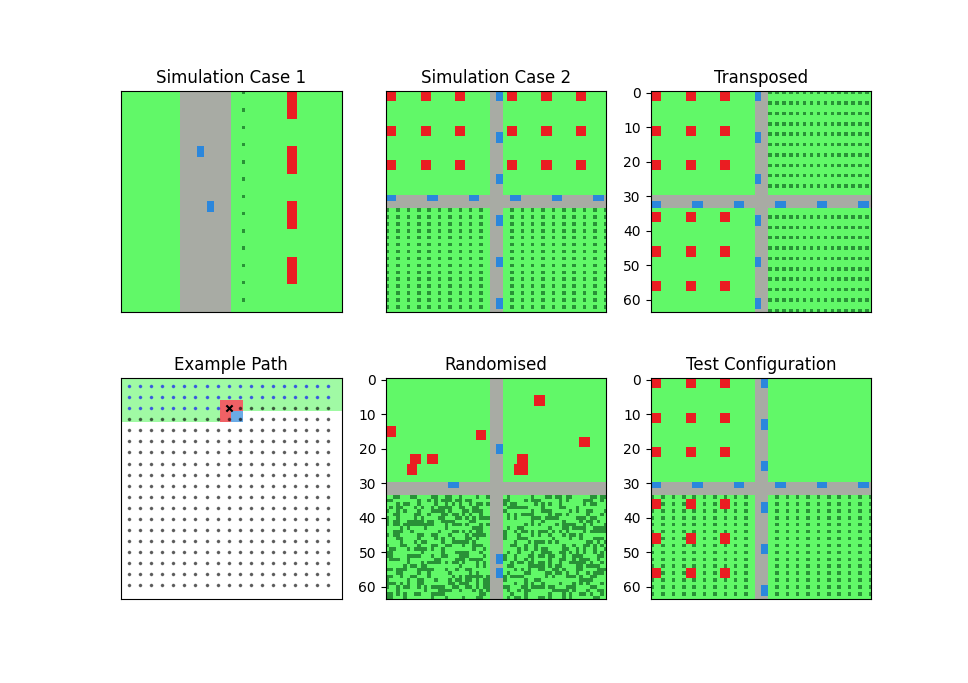
\includegraphics[width=4in]{SimComp10.png}}
    \caption{\bf{
        Example of the different test configurations. Colors represent different semantic classes. The top left corner shows the first simulation environment, the bottom left corner an example path. The top centre shows the second environment, the top right a transposed configuration, bottom centre a randomised configuration and bottom right a test configuration, which includes a partial tranpose.
    }}
    \label{fig:SimCase}
\end{figure*}
Figure~\ref{fig:SimCase} shows the basic variations for the simulation environments. The top left is the first environment, which is also used for the Monte-Carlo simulations detailed in section~\ref{ssec:MetMC} and excluded from the evaluation. The top centre shows the second environment, with the top right a transposed environment. The bottom left shows an example path, with the green colour indicating the already explored areas, the red the already seen fields and the blue the yet unexplored fields, which are predicted. The bottom centre shows a case where the placement of objects within their quadrants is randomised. The bottom right shows a testcase with partial transpose, which convolutes the definition of an ''area'' as a section identifiable by its composition of objects. The colours are indicators of types of classes and can be interpreted as shown in table~\ref{tab:colors}, however, are not limited to the named classes.
\begin{table}[]
    \renewcommand{\arraystretch}{1.3}
    \caption{\bf Color indicators}
    \label{tab:colors}
    \centering
    \begin{tabular}{|r||l|}
        \hline
        \bfseries Color      & \bfseries Class Name    \\
        \hline \hline
        Red &  House\\
        \hline
        Gray  & Road         \\
        \hline
        Light Green     & Grass              \\
        \hline
        Dark Green & Tree           \\
        \hline
        Blue & Vehicle \\
        \hline
    \end{tabular}
\end{table}

\subsubsection{Monte-Carlo simulations} \label{ssec:MetMC}
$1000$ simulations with fixed $o=0.5$, $f=2$ and
\begin{equation}
    p(z\mid x)=
    \begin{cases}
        0.8,~\text{for}~k=x \\
        \frac{1-0.8}{K-1},~\text{otherwise}
    \end{cases}
\end{equation}
are run on the first environment. $p(u)$ and $p(x\mid u)$ are sampled from a simplex and the performance of each algorithm as defined in section~\ref{ssec:MetEval} is recorded and the paramaters are saved if:
\begin{enumerate}
    \item The log-likelihood is smaller than the current smallest
    \item The difference between the predicted algorithm and the dynamic algorithm is bigger than the current biggest
\end{enumerate}
The final best results are used as parameters for simulations as defined in section~\ref{ssec:MetSim}.
\subsubsection{Evaluation}\label{ssec:MetEval}
To evaluate the reproduction quality of the posterior map for each individual state, the sum over the log-likelihoods for each cell $m_{i,j}$, defined by:
\begin{equation} \label{eq:Entropy}
    H_{i,j} = - \sum_{k} p_{i,j,k}~ln(q_{i,j,k})
\end{equation}
is used. $p_i$ represents the true state and $q_i$ the estimated map state. Furthermore, the number of wrongly predicted cells is calculated as a secondary indicator.
The log-likelihoods for the individual cases are subtracted from another and the count of the positive and negative samples indicate the relative quality of the reproduction for the different simulation environment. If the count is below $50$\%, the proposed solution performs worse. The metric is chosen as a robust indicator, which is not affected by large variances in individual cases. 
Only the second simulation case is included in the evaluation, since the first simulation environment was used to generate the updated probability vectors.
\section{Results} \label{sec:Res}
\subsection{Literature Overview} \label{ssec:ResLit}
\todo{Put figure here with the literature}
The semantic information in robotics is included on various levels, especially in the contemporary literature, without explicit definition
\begin{enumerate}
    \item Area
    \item Region
    \item Object
\end{enumerate}
Semantics, as study of signs, has far-reaching roots in language. Computer scientists working with language have put large efforts into attempting to model spoken and written language. Spoken language has employed Hierarchical models of language to separate spoken words (through HHMMs). Natural Language processing has looked deep and hard into classifying collections of words into topics and documents (which are considered mixtures of topics) for classification and proposition.
What we are currently missing from these are the reliable amounts of ground-truth data.
In speech applications: Various forms of Hierarchical Hidden Markov Models, mostly elucidated by Kevin Murphy~\todo{Cite his PhD Thesis here}
\subsubsection{Historic Literature} \label{sssec:ResLitHist}
The association of sensory inputs with symbolic systems and intricate representations has been discussed from a cognitive viewpoint by Harnad et al.~\cite{harnad_symbol_1990}.\\
Chown and colleagues~\cite{chown_prototypes_1995} researched the "what" and "where" subsystems of the human cognition and their learning over time. They captured the influence of landmark recognition, recreation of consistent Euclidean maps, as well as the importance of gateways, representing transitions between regions.\\
Kuipers~\cite{kuipers_spatial_2000} connected places, defined as 0D points, through 1D paths with 2D regions in topological maps. The proposed maps had a sensory and control level, a causal level, a topological level and a metrical level, all of which were connnected hierarchically.\\ Kuipers et al.~\cite{kuipers_local_2004} also conducted experiments where local metric room representations were linked through topological constraints.\\
Galindo et al.~\cite{galindo_robot_2008} connected a spatial hierarchical representation consisting of areas and objects with a terminological box and connected between these two in a deterministic manner to enable inference and path planning.\\
Borkowski et al.~\todo{Cite borkowski} assigned a hierarchical place taxomony based on architectural house representations to a metric map and performed path-planning within this map while considering semantic constraints.\\
Tenorth~\cite{tenorth_knowrob-map_2010} built a topological representation of abstract objects and locations and associates these in a hierarchical fashion to enhance task planning by incorporating the relations of objects.\\
Krishnan and Krishnan~\cite{krishnan_visual_2010} constructed a hierarchical semantical-topological and explored the semantic nodes before proceeding to the next one, making use of transition areas as mentioned in~\cite{chown_prototypes_1995}.
\subsection{Contemporary Literature} \label{sssec:ResLitCont}
Contemporary image processing techniques have accelerated semantic spatial research through significant improvements in reliability and robustness of classification and localisation~\cite{alom_history_2018}.\\
Suenderhauf et al.~\cite{sunderhauf_meaningful_2017} associated point-clouds in SLAM with labels propagated through a modern neural network.\\
Zhang et al.~\cite{zhang_hierarchical_2019} used a hierarchical topic model to improve the performance of a SLAM system by actively integrating the object association problem into a hierarchical dirichlet process.\\
Yang et al.~\cite{yang_visual_2018} used scene priors derived from vector representations of class names to enhance a reinforcement learning module which relies on visual cues in indoor environments.\\
Wu et al.~\cite{wu_learning_2018} used reinforcement learning to train an agent to recognise a room and infer whether another room type is directly accessible from this room using a bernoulli distribution.\\
Chaplot et al.~\cite{chaplot_object_2020} won the 2020 CVPR challenge to navigate to an object goal by learning a semantic-metric map from visual cues and training a policy to generate frontier-based goals. Their research also highlighted that other RL policies were outperformed by frontier-based methods and were unable to generalize to the real-world.\\
\subsection{UAV Literature} \label{sssec:ResLitUAV}
UAV-based systems present different approaches to including semantic information. A substantial amount of literature is concerned with passive acquisition of semantic information.\\
Le Saux and Sanfourche~\cite{saux_rapid_2013}, Sheppard and Rahnemoonfar~\cite{sheppard_real-time_2017}, Christie et al.~\cite{christie_semantics_2016} and Kyrkou et al.~\cite{kyrkou_dronet:_2018}, classified top-down images taken from a UAV in real-time with respect to different classes and approaches. \\
Cavaliere et al.~\cite{cavaliere_towards_2016,cavaliere_towards_2018} associated ''tracks'' coming from images with ''places'' from geospatial information to describe relations between them in a relational manner, as detailed in~\cite{landsiedel_review_2017}. The individual items were structured hierarchically to distinguish between different type of tracks, such as vehicles and humans on the first level and cars, motorcycles and trucks on the second level.\\
Drouilly et al.~\cite{drouilly_semantic_2015} developed a metric to evaluate the semantic quality of a path through an environment depending on the distribution of objects and the observation quality.

Semantic information has also been actively employed in navigation algorithms to enhance their performance.\\
Maturana et al.~\cite{maturana_looking_2017} annotated a 2.5D map with detection of cars to approach these.\\
Maravall et al.~\cite{maravall_navigation_2017} used the image entropy to navigate through a topological map to semantically salient places.\\
Alirezaie~\cite{alirezaie_exploiting_2017} developed a RRT implementation that discards semantically inadmissible points through geospatial information associated with the waypoints and significantly improved planning time for longer distances.\\
Dang et al.~\cite{dang_autonomous_2018} employed an object detector on top of a voxel grid to detect humans and bicycles.\\
Koch et al.~\cite{koch_automatic_2019} respected semantic constraints during the path planning step for 3D reconstruction using UAVs while maintaining the quality of the reconstruction.
Toudeshki et al.~\cite{toudeshki_robust_2018} combined a visual teach-and-repeat approach with an object detector to funnel the UAV to follow a path.
% \subsection{Literature on Hierarchical models from NLP}
\subsection{Open Problems for semantic UAV navigation} \label{ssec:ResOpen}
Problem: "Gateways" as defined by Chown~\cite{chown_prototypes_1995}, used by Kuipers~\cite{kuipers_local_2004}, Krishnan and Krishan~\cite{krishnan_visual_2010} and Wu et al.~\cite{wu_learning_2018} for successful implementations are difficult outdoors - where a room ends is quite easy (with a door/window), but where does the lawn end and the golf court begin? \\
Problem: RL are not capable of generalizing well~\cite{chaplot_object_2020} and also do not consistently outperform generalized path planning.\\
Problem: UAV viewpoints provide a hurdle for use of off-the-shelf NNs~\cite{richardwebster_psyphy:_2019}.\\
Problem: UAV path-planning is often done in a way to reliably cover large areas~\cite{vanegas_novel_2018}.\\
Task definition is difficult, see Anderson et al.~\cite{anderson_evaluation_2018}.
Challenges and unified datasets as the drivers~\cite{corke_what_2020} for semantic tasks for UAVs are difficult to acquire. Racing has recently largely benefitted from clear definition of tasks and the performance increases have been shown to be tremendous.
\todo{Include possible remedies from Natural Language Processing}

\subsection{Simulations} \label{ssec:ResSim}
\todo{Throw the number of total simulations run in here}
Figure~\ref{fig:Res} displays the results of the numerical simulations, only evaluated on the second simulation case. The value indicates the percentage of cases where the proposed method outperformed the second best algorithm, where the mixing parameter was employed to update the prior. Both of these algorithms consistently outperformed the baseline.  
\begin{figure*}
    \centering
    \resizebox{\textwidth}{!}{
    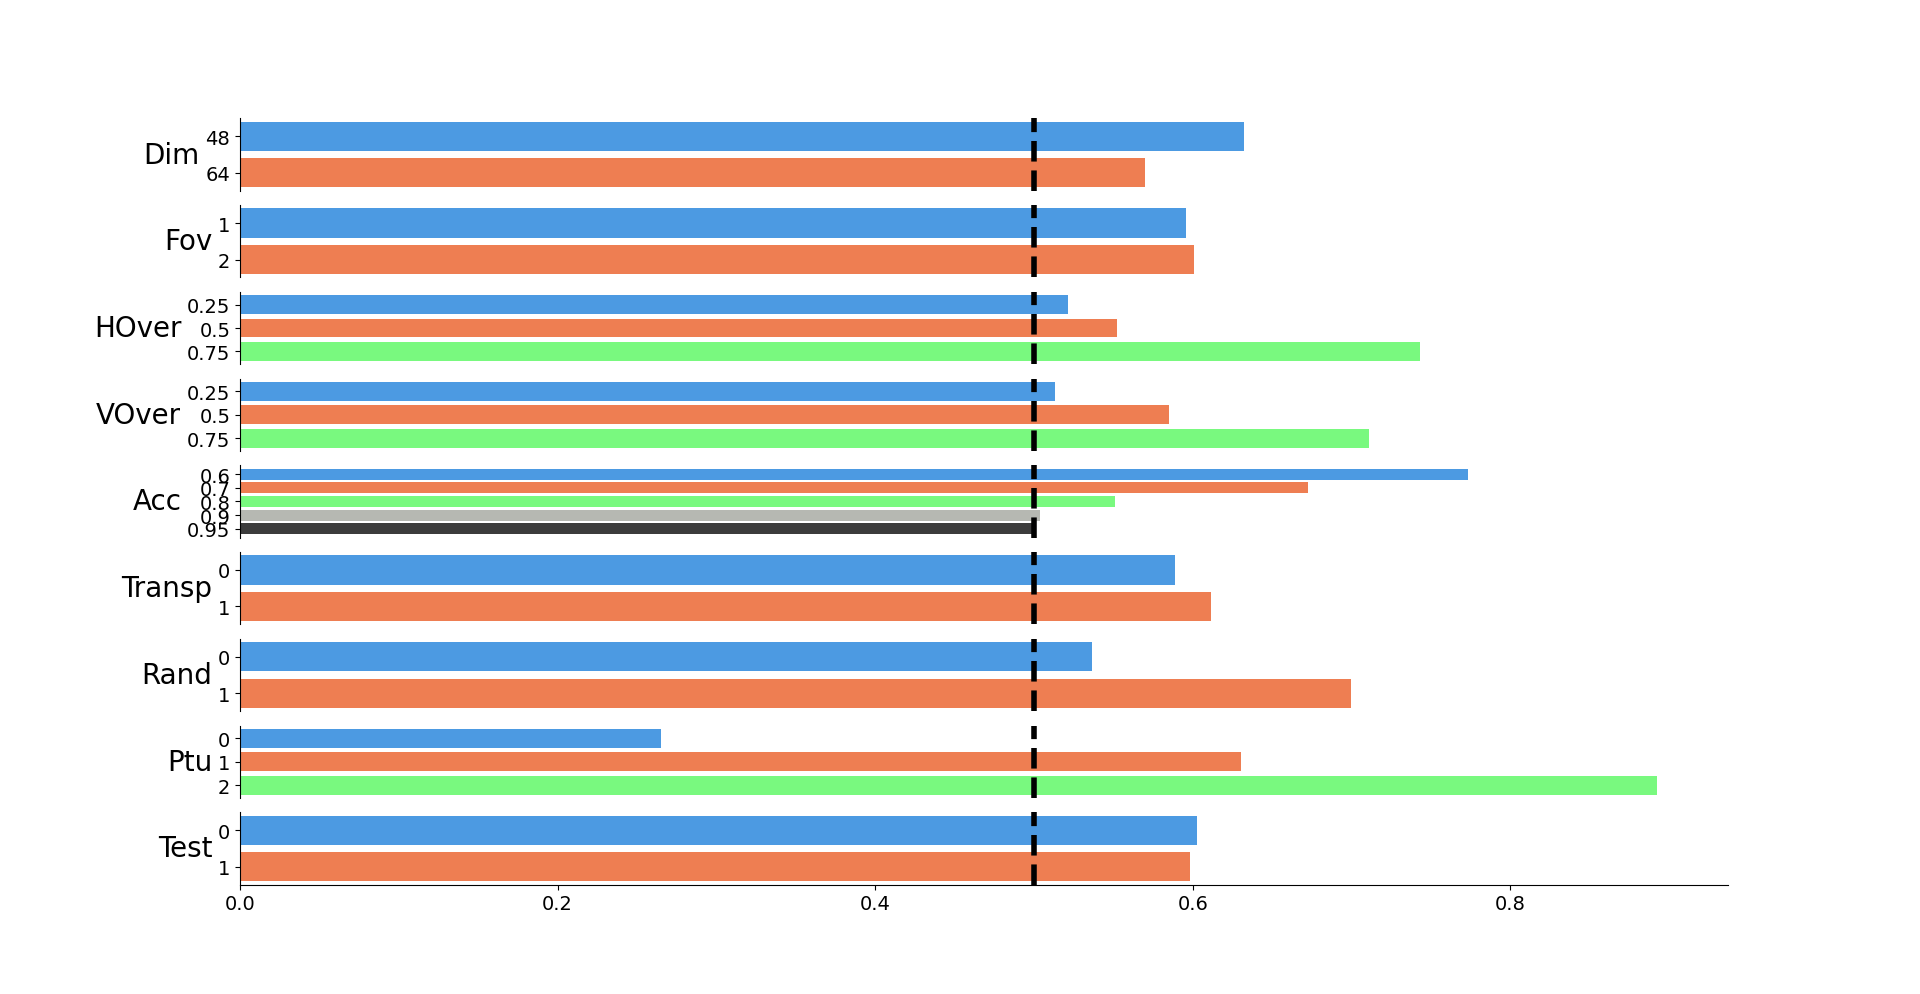
\includegraphics[width=4in]{Results-10.png}}
    \caption{\bf{
        Relative amount of cases where the entropy for dynamically updated priors was lower than for linear mixing. The black vertical line indicates the $50$ threshold. Values lower than the threshold indicate a worse perforamnce.
    }}
    \label{fig:Res}
\end{figure*}
The decreasing bars for accuracy in figure~\ref{fig:Res} indicate that the influence of the prior diminishes when the detection accuracy improves, which is aligned with the intuition of bayesian filtering, as the detections converge. The increasing performance with increasing overlap shows that additional observations increase the robustness of the algorithm. The low value for Ptu case 0 shows that a handcrafted mixing parameter performs significantly worse, however, the high values for 1 and 2 indicate that with the right choice of parameters, the performance can increase significantly. This still holds true for cases where the placement of objects is randomized, as well as cases where a convolution of areas has taken place.~\todo{reference back to the image of a single test case here}. The Transp-row indicates that the alignment of axes of the map with the path planning do not have a significant influence on the performance.

\section{Discussion} \label{sec:Disc}
\begin{itemize}
    \item Simplified simulation serves as an indicator of performance
    \item Test cases are lacking
    \item Clear definitons of areas are lacking
    \item example of successful application are Fei-Fei-Lis LDA Application, and the other ones for the scenes and images. And the one with the satellite images. Maybe we can use these to turn into sophisticated models?
\end{itemize}

\section{Future Work} \label{sec:Fut}
\begin{itemize}
    \item Adopting models that have proven to be successful in language (such as LDA)
    \item Test Configuration
\end{itemize}
%%%%%%%%%%%%%%%%%%%%%%%%%%%%%%%%%%%%%%%%%%%%%%%%%%%%%%%%%%%%%%%%%%%%%%%%%%%%%%%%%%%%%%%%%%%%%%%%%
\appendices{}              % note there is no {} to put a title. Each appendix has its own title
%%%%%%%%%%%%%%%%%%%%%%%%%%%%%%%%%%%%%%%%%%%%%%%%%%%%%%%%%%%%%%%%%%%%%%%%%%%%%%%%%%%%%%%%%%%%%%%%%
% For a single appendix, use the \appendix{} keyword and do not use the \section command.

\section{More Information}        % first appendix
%%%%%%%%%%%%%%%%%%%%%%%%%%
This is the first appendix.

\subsection{Comments}
If you have only one appendix, use the ``appendix'' keyword.

\subsection{More Comments}
Use section and subsection keywords as usual.

\section{Yet More Information}    % second appendix
%%%%%%%%%%%%%%%%%%%%%%%%%%%%%%
This is the second appendix.



%%%%%%%%%%%%%%%%%%%%%%%%%%%%%%%%%%%%%%%%%%%%%%%%%%%%%%%%%%%%%%%%%%%%%%%%%%%%%%%%%%%%%%%%%%%%%%%%%%%%%%
\acknowledgments
The authors thank the Office of Naval Research for funding this project.



%%%%%%%%%%%%%%%%%%%%%%%%%%%%%%%%%%%%%%%%%%%%%%%%%%%%%%%%%%%%%%%%%%%%%%%%%%%%%%%%%%%%%%%%%%%%%%%%%%%%%%
\bibliographystyle{IEEEtran}
\bibliography{references}


%%%%%%%%%%%%%%%%%%%%%%%%%%%%%%%%%%%%%%%%%%%%%%%%%%%%%%%%%%%%%%%%%%%%%%%%%%%%%%%%%%%%%%%%%%%%%%%%%%%%%%
\thebiography
%% This biostyle allows you to insert your photo size 1in X 1.25in
\begin{biographywithpic}{Nicolas Mandel}{blankpic.eps}
    Blablabla
\end{biographywithpic}

\begin{biographywithpic}{Michael}{blankpic.eps}
    Blablabla
\end{biographywithpic}




\end{document}
